\documentclass[crop,tikz]{standalone}

\begin{document}
	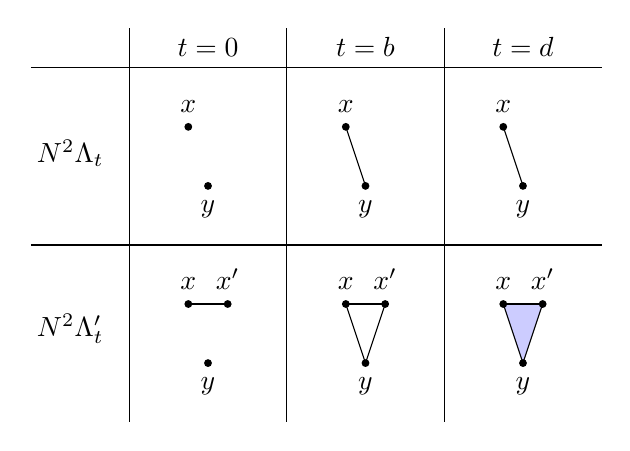
\begin{tikzpicture}
	% Čech nerve t=0
	\node[circle,inner sep=1pt,fill=black,label=above:{$x$}] at (0,-0.25) {};
	\node[circle,inner sep=1pt,fill=black,label=below:{$y$}] at (0.25,-1) {};

	% Čech nerve t=l
	\draw (2,-0.25) -- (2.25,-1);
	\node[circle,inner sep=1pt,fill=black,label=above:{$x$}] at (2,-0.25) {};
	\node[circle,inner sep=1pt,fill=black,label=below:{$y$}] at (2.25,-1) {};
	
	% Čech nerve t=2l
	\draw (4,-0.25) -- (4.25,-1);
	\node[circle,inner sep=1pt,fill=black,label=above:{$x$}] at (4,-0.25) {};
	\node[circle,inner sep=1pt,fill=black,label=below:{$y$}] at (4.25,-1) {};
	
	% p nerve t=0
	\draw (0,-0.25-2.25) -- (0.5,-0.25-2.25);
	\node[circle,inner sep=1pt,fill=black,label=above:{$x$}] at (0,-0.25-2.25) {};
	\node[circle,inner sep=1pt,fill=black,label=above:{$x'$}] at (0.5,-0.25-2.25) {};
	\node[circle,inner sep=1pt,fill=black,label=below:{$y$}] at (0.25,-1-2.25) {};
	
	% p nerve t=l
	\draw (2,-0.25-2.25) -- (2.5,-0.25-2.25);
	\draw (2,-0.25-2.25) -- (2.25,-1-2.25);
	\draw (2.5,-0.25-2.25) -- (2.25,-1-2.25);
	\node[circle,inner sep=1pt,fill=black,label=above:{$x$}] at (2,-0.25-2.25) {};
	\node[circle,inner sep=1pt,fill=black,label=above:{$x'$}] at (2.5,-0.25-2.25) {};
	\node[circle,inner sep=1pt,fill=black,label=below:{$y$}] at (2.25,-1-2.25) {};
	
	% p nerve t=2l
	\fill[fill=blue!20] (4,-0.25-2.25) -- (4.5,-0.25-2.25) -- (4.25,-1-2.25);
	\draw (4,-0.25-2.25) -- (4.5,-0.25-2.25);
	\draw (4,-0.25-2.25) -- (4.25,-1-2.25);
	\draw (4.5,-0.25-2.25) -- (4.25,-1-2.25);
	\node[circle,inner sep=1pt,fill=black,label=above:{$x$}] at (4,-0.25-2.25) {};
	\node[circle,inner sep=1pt,fill=black,label=above:{$x'$}] at (4.5,-0.25-2.25) {};
	\node[circle,inner sep=1pt,fill=black,label=below:{$y$}] at (4.25,-1-2.25) {};
	
	% Grid
	\draw (-0.75,1) -- (-0.75,-4);
	\draw (1.25,1) -- (1.25,-4);
	\draw (3.25,1) -- (3.25,-4);
	\draw (-2,0.5) -- (5.25,0.5);
	\draw (-2,-1.75) -- (5.25,-1.75);
	
	% Top labels
	\node[label=above:{$t=b$}] at (2.25, .4) {};
	\node[label=above:{$t=0$}] at (0.25, .4) {};
	\node[label=above:{$t=d$}] at (4.25, .4) {};
	
	% Left labels
	\node[label=above:{$N^2\Lambda_t$}] at (-1.5, -1) {};
	\node[label=above:{$N^2\Lambda'_t$}] at (-1.5, -3.25) {};

	\end{tikzpicture}
\end{document}